\documentclass[leqno]{article}
% Shared QBT/Soln pack preamble for resources.danieljsmith.org.
\usepackage{graphicx}
\usepackage{dsfont}
\usepackage{mathtools}
\usepackage{amssymb}
\usepackage{amsmath}
\usepackage{mleftright}
\usepackage{amsthm}
\usepackage{float}
\usepackage{ragged2e}
\usepackage{tensor}
\usepackage{fancyhdr}
\usepackage{empheq}
\usepackage[most]{tcolorbox}
\usepackage{enumitem}
\usepackage{dirtytalk}
\usepackage{marginnote}
\usepackage{microtype}
\usepackage[
  a4paper,
  left=0.8in,
  right=1in,
  top=1in,
  bottom=0.5in,
  headheight=14pt,
  headsep=0.4in
]{geometry}
\setlength{\parindent}{0cm}

% TikZ / PGFPlots
\usepackage{pgfplots}
\pgfplotsset{compat=1.18}
\usepgfplotslibrary{fillbetween, polar}
\usetikzlibrary{calc, positioning}
\usetikzlibrary{angles, quotes}
\usetikzlibrary{arrows.meta}
\usetikzlibrary{decorations.pathreplacing, decorations.markings}
\usetikzlibrary{patterns}
\usetikzlibrary{intersections}

% Links and contents. The contents follow the TMUA papers: compact entries,
% no dot leaders, and each question's mark total in grey after its label.
\usepackage{tocloft}
\tocloftpagestyle{fancy}
\setlength{\cftbeforesubsecskip}{2pt}
\setlength{\cftsubsecindent}{1.5em}
\setlength{\cftsubsecnumwidth}{0pt}
\renewcommand{\cftsubsecfont}{\small\color{black}}
\renewcommand{\cftsubsecpagefont}{\small\color{black}}
\renewcommand{\cftsubsecleader}{\hfill}
\usepackage[colorlinks=true,linkcolor=black,citecolor=magenta,urlcolor=black]{hyperref}%
\urlstyle{same}

% Pack macros
% \marks also adds its value to the current question's total in the .aux
% file, so the contents show each total from the second pass. The write
% happens at shipout, so a box typeset more than once counts once. The
% pack's mark total for the contents-page title is summed the same way.
\makeatletter
\newcount\djs@totalmarks
\newcommand{\djsAddMarks}[2]{%
  \global\advance\djs@totalmarks#2\relax
  \@ifundefined{djs@marks@#1}%
    {\expandafter\xdef\csname djs@marks@#1\endcsname{#2}}%
    {\expandafter\xdef\csname djs@marks@#1\endcsname
      {\the\numexpr\csname djs@marks@#1\endcsname+#2\relax}}}
\RenewDocumentCommand{\marks}{o m}{%
  \protected@write\@auxout{}{\string\djsAddMarks{\number\value{enumi}}{#2}}%
  \IfValueTF{#1}%
    {\marginnote{\raggedright\textbf{[#2]}}[#1]}%
    {\marginnote{\raggedright\textbf{[#2]}}}%
}
\makeatother

\newcommand{\vspacerule}[2]{%
  \par\vspace*{#1}%
  \noindent\hrulefill\par
  \vspace*{#2}%
}

\definecolor{scarlet}{RGB}{205, 40, 75}
% Site colours for the contents-page title: the accent, the rule colour, a
% stronger rule colour for the path separator, and the muted text colour.
\definecolor{djsBurgundy}{RGB}{118, 59, 67}
\definecolor{djsHairline}{RGB}{216, 213, 205}
\definecolor{djsSlash}{RGB}{170, 166, 158}
\definecolor{djsMuted}{RGB}{96, 101, 106}

% Worked-solution box, adapted from the TMUA worked-solutions box. A white breakable box with a left scarlet rule and no surrounding
% frame or tint. A part that breaks fills the rest of its page, so the rule
% runs to the bottom margin; the unbroken or last part ends in a short
% horizontal foot rule so a solution visibly stops. Unlike the TMUA box there
% is no answer label. The box does not grow to the left, so the rule sits at
% the text edge; growing to the right keeps the usable line width close to the
% old tcolorbox Solution box.
% Spacing inside the box: paragraphs are 6pt apart, so source blank lines show
% (solutions put one after each display and none between a lead-in and its
% display). Every display gets 6pt above and 10pt below, whatever the length
% of its lead-in line; align rows are spread by an 8pt \jot; solution parts
% are 14pt apart and sub-parts 8pt; \left and \right space like ordinary
% brackets (mleftright); no single line is stranded at a page break; and
% neither the Solution label nor the line before a list ends a page. No
% skip can shrink, so full pages are not squeezed.
\newtcolorbox{djsSolution}{%
  enhanced, breakable, frame hidden, sharp corners, colback=white,
  height fixed for=first and middle, height fill,
  extras unbroken and last={natural height},
  borderline west={2.2pt}{0pt}{scarlet},
  left=11pt, right=0pt, top=5pt, bottom=13pt,
  before skip=13pt, after skip=4pt,
  grow to right by=10mm,
  overlay unbroken and last={%
    \fill[scarlet] (frame.south west)
      rectangle ([xshift=3.5cm, yshift=2.2pt]frame.south west);},
  before upper={{\color{scarlet}\bfseries Solution}\par\nobreak\vspace{4pt}%
    \setlength{\parskip}{6pt plus 2pt}%
    \setlength{\abovedisplayskip}{6pt plus 2pt}%
    \setlength{\abovedisplayshortskip}{6pt plus 2pt}%
    \setlength{\belowdisplayskip}{10pt plus 2pt}%
    \setlength{\belowdisplayshortskip}{10pt plus 2pt}%
    \setlength{\jot}{8pt}%
    \setlist{parsep=6pt plus 2pt, topsep=6pt plus 2pt, beginpenalty=10000}%
    \setlist[enumerate,1]{itemsep=14pt plus 2pt}%
    \setlist[enumerate,2]{itemsep=8pt plus 2pt}%
    \mleftright
    \clubpenalty=10000 \widowpenalty=10000 \displaywidowpenalty=10000\relax}}

% Optional smaller figure inside a solution box. \scalebox shrinks node text
% with the drawing. Not applied to existing figures.
\newcommand{\SolnFigureScale}{0.85}
\newsavebox{\djsSolnFigureBox}
\newenvironment{djsSolutionFigure}
  {\par\vspace{4pt}\begin{center}\begin{lrbox}{\djsSolnFigureBox}}
  {\end{lrbox}\scalebox{\SolnFigureScale}{\usebox{\djsSolnFigureBox}}%
   \end{center}\vspace{2pt}\par}

\newcommand{\cxl}[2]{%
  \tikz[baseline=(X.base)]{%
    \node[inner sep=0pt, outer sep=0pt, text=#1] (X) {$#2$};
    \draw[#1, line width=0.4pt] (X.south west)--(X.north east);
  }%
}

% Page-style hook run at the contents page and each question's opening page.
% A no-op for QBT packs; \djsSolnHeader points it at the fancy header.
\newcommand{\djsQuestionPageStyle}{}

% A contents entry: "Question N" in a box wide enough for two digits, so the
% mark totals line up, then the total in grey. Bookmarks keep "Question N".
\makeatletter
\newlength{\djsTocLabelWidth}
\newcommand{\djsTocMarks}[1]{%
  \@ifundefined{djs@marks@#1}{}{%
    {\footnotesize\itshape\color{black!45}%
     \csname djs@marks@#1\endcsname~mark%
     \ifnum\csname djs@marks@#1\endcsname=1 \else s\fi}}}
\newcommand{\djsTocEntry}[1]{%
  \texorpdfstring
    {\settowidth{\djsTocLabelWidth}{Question 00}%
     \makebox[\dimexpr\djsTocLabelWidth+0.9em\relax][l]{Question #1}%
     \djsTocMarks{#1}}%
    {Question #1}}
\makeatother

% The question count for the contents-page title is written to the .aux at
% the end of the document, so it also appears from the second pass.
\newcounter{djsQuestions}
\newcommand{\questionitem}{%
  \djsQuestionPageStyle
  \item\phantomsection
  \stepcounter{djsQuestions}%
  \addcontentsline{toc}{subsection}{\protect\djsTocEntry{\number\value{enumi}}}%
}
\makeatletter
\newcommand{\djsSetQuestionCount}[1]{\gdef\djs@questioncount{#1}}
\AtEndDocument{\immediate\write\@auxout
  {\string\djsSetQuestionCount{\number\value{djsQuestions}}}}
\makeatother

\renewcommand{\contentsname}{Questions}

% \djsPackHeader[<link content tag>]{<left header>}; the tag says which
% document a click on the header link came from.
\newcommand{\djsPackHeader}[2][questions]{%
  \pagestyle{fancy}%
  \fancyhead{}%
  \fancyfoot{}%
  \renewcommand{\headrulewidth}{0.9pt}%
  \lhead{#2}%
  \chead{}%
  \rhead{\href{https://danieljsmith.org/?utm_source=pdf&utm_campaign=further-maths&utm_content=#1}{danieljsmith.org}}%
}

% The header's topic is also the contents-page title, under which a label
% says which booklet this is.
\newcommand{\djsPackTitle}{}
\newcommand{\djsBookletLabel}{}
\newcommand{\djsQbtHeader}[1]{%
  \djsPackHeader{#1}%
  \renewcommand{\djsPackTitle}{#1}%
  \renewcommand{\djsBookletLabel}{Questions by topic}%
}

% The colophon at the foot of page one, independent of the page style: the
% contents-page title's hairline led by a short scarlet rule, then the date on
% the left and a link to the site on the right, all inside the bottom margin.
% Its sizes are fixed, so it matches the TMUA papers' colophon. The document
% supplies the date; recompiling never changes it.
\makeatletter
\newcommand{\djsLastUpdated}[1]{%
  \AtBeginDocument{\AddToHookNext{shipout/foreground}{\djs@colophon{#1}}}}
\newcommand{\djs@colophon}[1]{%
  \put(0.8in,-\dimexpr\paperheight-0.47in\relax){%
    \makebox[0pt][l]{\color{djsHairline}%
      \rule[0.9pt]{\dimexpr\paperwidth-1.8in\relax}{0.6pt}}%
    \makebox[0pt][l]{\color{scarlet}\rule{3.5cm}{2.2pt}}}%
  \put(0.8in,-\dimexpr\paperheight-0.32in\relax){\makebox[0pt][l]{%
    \fontsize{9}{11}\selectfont Last updated #1}}%
  \put(\dimexpr\paperwidth-1in\relax,-\dimexpr\paperheight-0.32in\relax){%
    \makebox[0pt][r]{\fontsize{7}{8.5}\selectfont\color{djsMuted}%
      Latest version at \href{https://resources.danieljsmith.org/}%
        {\color{black}resources.danieljsmith.org}}}}
\makeatother

% Solutions packs show the header only on the contents page and each
% question's opening page, so it never appears part-way through a solution.
% \thispagestyle marks the next page shipped out, which is the question's
% page because every solution question starts after a \newpage.
\newcommand{\djsSolnHeader}[1]{%
  \djsPackHeader[solutions]{\textit{Solutions} - #1}%
  \pagestyle{empty}%
  \renewcommand{\djsQuestionPageStyle}{\thispagestyle{fancy}}%
  \renewcommand{\djsPackTitle}{#1}%
  \renewcommand{\djsBookletLabel}{Worked solutions}%
}

% \djsSitePath{<strand>}{<topic>}, called once after the header, names where
% the pack sits on the site; the contents-page title prints it above the pack
% title, e.g. CORE PURE / FURTHER CALCULUS. Without it the line is left out.
\makeatletter
\newif\ifdjs@sitepath
\newcommand{\djs@strand}{}
\newcommand{\djs@section}{}
\newcommand{\djsSitePath}[2]{%
  \djs@sitepathtrue
  \renewcommand{\djs@strand}{#1}%
  \renewcommand{\djs@section}{#2}%
}
\makeatother

% Further Mechanics packs call \djsMechanicsPack in their preamble, so that
% \djsFrontMatter prints the default value of g above the contents. The box
% keeps its own space above it (before skip is the whole gap below the title,
% not an addition to it). Without the box, \djsGravityNote is just extra space
% before the contents heading, bringing the gap above it close to the gap
% between the box and the heading on Further Mechanics pages.
\newcommand{\djsGravityNote}{\vspace{14pt}}
\newcommand{\djsMechanicsPack}{%
  \renewcommand{\djsGravityNote}{%
    \begin{tcolorbox}[sharp corners, colback=white, colframe=black,
      boxrule=1pt, left=8pt, right=8pt, top=6pt, bottom=6pt,
      before skip=20pt]
    {\bfseries Instructions}\par\vspace{4pt}
    Unless a question states otherwise, take $g = 9.8\,\mathrm{m\,s^{-2}}$
    wherever a numerical value of $g$ is required. Solutions also give final
    answers for $g = 10\,\mathrm{m\,s^{-2}}$ where these differ.
    \end{tcolorbox}%
    \vspace{16pt}}%
}

% Contents-page title: the site path in spaced burgundy capitals, the pack
% title, a hairline led by a short scarlet rule (the solution box's foot rule),
% then the booklet label with the question and mark counts. The counts come
% from the .aux, so they appear from the second pass.
\makeatletter
\newsavebox{\djs@eyebrowbox}
\newcommand{\djs@caps}[1]{\textls[180]{\MakeUppercase{#1}}}
\newcommand{\djs@eyebrow}{%
  \color{djsBurgundy}\footnotesize\bfseries
  \djs@caps{\djs@strand}%
  {\color{djsSlash}\hspace{0.55em}/\hspace{0.55em}}%
  \djs@caps{\djs@section}}
\newcommand{\djs@dot}{\hspace{0.45em}\textperiodcentered\hspace{0.45em}}
\newcommand{\djs@counts}{%
  \@ifundefined{djs@questioncount}{}{%
    \djs@questioncount~question\ifnum\djs@questioncount=1 \else s\fi
    \ifnum\djs@totalmarks>0
      \djs@dot\the\djs@totalmarks~mark\ifnum\djs@totalmarks=1 \else s\fi
    \fi}}
\newcommand{\djsContentsTitle}{%
  \ifdjs@sitepath
    \sbox\djs@eyebrowbox{\djs@eyebrow}%
    \ifdim\wd\djs@eyebrowbox>\linewidth
      \@latex@warning@no@line{The \string\djsSitePath\space line is wider
        than the text, so it wraps. Shorten its topic}%
    \fi
    {\raggedright\djs@eyebrow\par}%
    \vspace{7pt}%
  \fi
  {\raggedright\fontsize{24.88}{28}\selectfont\djsPackTitle\par}%
  \vspace{9pt}%
  \noindent\makebox[0pt][l]{\color{djsHairline}\rule[0.9pt]{\linewidth}{0.6pt}}%
  {\color{scarlet}\rule{3.5cm}{2.2pt}}\par
  \vspace{5pt}%
  {\small\color{djsMuted}\djsBookletLabel\hfill\djs@counts\par}%
  \vspace{8pt}%
}
\makeatother

\newcommand{\djsFrontMatter}{%
  \djsQuestionPageStyle
  \vspace*{6pt}%
  \djsContentsTitle
  \djsGravityNote
  \tableofcontents
  \newpage
}


\djsSolnHeader{Centre of Mass of Composite Solids}
\djsSitePath{Further Mechanics}{Centre of Mass}
\djsMechanicsPack
\djsLastUpdated{27 October 2026}

\begin{document}
\djsFrontMatter
\begin{enumerate}[
  label=\textbf{\arabic*.},
  leftmargin=*,
  topsep=0pt,
  partopsep=0pt,
  parsep=0pt
]

% ---- Question 1 ----
\questionitem
% [Source: _QBT___Solns__Centre_of_Mass_of_Composite_Solids, Q1]

\begin{figure}[H]
\centering
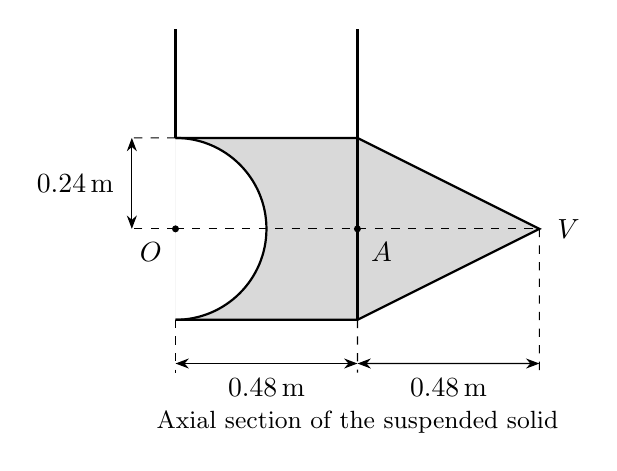
\begin{tikzpicture}[scale=1.05,
  dimension/.style={{Stealth[length=1.7mm]}-{Stealth[length=1.7mm]}}]
\def\rad{1.1}
\pgfmathsetmacro{\cylLength}{2*\rad}
\pgfmathsetmacro{\coneLength}{2*\rad}
\pgfmathsetmacro{\stringLength}{1.2*\rad}
\pgfmathsetmacro{\dimGap}{0.48*\rad}
\coordinate (O) at (0,0);
\coordinate (A) at (\cylLength,0);
\coordinate (V) at ({\cylLength+\coneLength},0);
\coordinate (T) at ($(O)+(0,\rad)$);
\coordinate (B) at ($(O)+(0,-\rad)$);
\coordinate (U) at ($(A)+(0,\rad)$);
\coordinate (D) at ($(A)+(0,-\rad)$);
\coordinate (DimO) at ($(B)+(0,-\dimGap)$);
\coordinate (DimA) at ($(D)+(0,-\dimGap)$);
\coordinate (DimV) at (V |- DimA);
\coordinate (RadO) at ($(O)+(-\dimGap,0)$);
\coordinate (RadT) at ($(T)+(-\dimGap,0)$);
\fill[gray!30] (T)--(U)--(V)--(D)--(B)--cycle;
\fill[white] (T) arc[start angle=90,end angle=-90,radius=\rad]--cycle;
\draw[thick] (T)--(U)--(V)--(D)--(B);
\draw[thick] (T) arc[start angle=90,end angle=-90,radius=\rad];
\draw[thick] (U)--(D);
\draw[dashed] (O)--(V);
\draw[thick] (T)--++(0,\stringLength);
\draw[thick] (U)--++(0,\stringLength);
\foreach \P in {O,A} {\fill (\P) circle (1.2pt);}
\node[below left=2pt] at (O) {$O$};
\node[below right=2pt] at (A) {$A$};
\node[right=3pt] at (V) {$V$};
\draw[dashed] (B)--($(DimO)+(0,-0.1*\rad)$);
\draw[dashed] (D)--($(DimA)+(0,-0.1*\rad)$);
\draw[dashed] (V)--($(DimV)+(0,-0.1*\rad)$);
\draw[dimension] (DimO)--node[midway,below=2pt] {$0.48\,\mathrm{m}$}(DimA);
\draw[dimension] (DimA)--node[midway,below=2pt] {$0.48\,\mathrm{m}$}(DimV);
\draw[dashed] (O)--(RadO);
\draw[dashed] (T)--(RadT);
\draw[dimension] (RadO)--node[midway,left=3pt] {$0.24\,\mathrm{m}$}(RadT);
\node[font=\small] at ($(DimA)+(0,-0.65*\rad)$) {Axial section of the suspended solid};
\end{tikzpicture}
\end{figure}


A solid cylinder has radius $0.24\,\mathrm{m}$ and length $0.48\,\mathrm{m}$. A hemispherical cavity of radius $0.24\,\mathrm{m}$ is cut into one end of the cylinder, with its circular opening coinciding with that end face. A solid cone of base radius $0.24\,\mathrm{m}$ and height $0.48\,\mathrm{m}$ is joined to the opposite end of the cylinder so that their circular faces coincide. \\

The resulting solid $S$ has uniform density throughout. Let $O$ be the centre of the opening of the cavity, $A$ the centre of the cylinder-cone joint and $V$ the vertex of the cone. The points $O$, $A$ and $V$ lie on the common axis, in that order. The centre of mass of $S$ is $G$. \\
You may use the following results for uniform solids:
\begin{itemize}[nosep]
\item A hemisphere of radius $r$ has volume $\frac{2}{3}\pi r^3$ and its centre of mass is $\frac38 r$ from its plane face towards its curved surface.
\item A cone of base radius $r$ and height $h$ has volume $\frac{1}{3}\pi r^2h$ and its centre of mass is $\frac14 h$ from its base towards its vertex.
\end{itemize}

\begin{enumerate}[label=\textbf{(\alph*)}]
\item Explain why $G$ lies on the line $OV$. \marks{1} \\
\item Find the distance $OG$. \marks{4} \\
\end{enumerate}
The solid is suspended by two light vertical strings. One is attached to the uppermost point of the circular rim centred at $O$, and the other to the uppermost point of the circular joint centred at $A$. The solid hangs in equilibrium with $OV$ horizontal, as shown in the diagram above. \\
\begin{enumerate}[label=\textbf{(\alph*)}, resume]
\item Given that the weight of $S$ is $W$, find the tension in each string in terms of $W$. \marks{3} \\
\end{enumerate}

\vspace*{10pt}

\begin{djsSolution}
\begin{enumerate}[label=\textbf{(\alph*)}, start=1]
\item The solid has uniform density and is rotationally symmetric about \(OV\), so its centre of mass lies on \(OV\).

\item Let \(r=0.24\,\mathrm{m}\) and let the density be \(\rho\). Both the cylinder's length and the cone's height are \(2r\). Measure distances along the axis from \(O\) towards \(V\).

The centre of mass of a uniform solid cylinder lies halfway along its axis.
The centre of mass of a uniform solid hemisphere of radius \(R\) lies on its axis, a distance \(\frac38 R\) from its plane face towards the curved surface.
The centre of mass of a uniform solid cone of height \(H\) lies on its axis, a distance \(\frac14 H\) from its base towards its vertex.

Using mass \(=\) density \(\times\) volume:
\[
\begingroup
\renewcommand{\arraystretch}{1.65}
\setlength{\arraycolsep}{10pt}
\begin{array}{c|c|c}
\text{Component} & \text{Mass} & \text{Axial distance from }O \\
\hline
\text{Complete cylinder} & m_1=\rho\pi r^2(2r)=2\rho\pi r^3 & x_1=r \\
\text{Removed hemisphere} & m_2=\frac23\rho\pi r^3 & x_2=\frac{3r}{8} \\
\text{Cone} & m_3=\frac13\rho\pi r^2(2r)=\frac23\rho\pi r^3 & x_3=2r+\frac{2r}{4}=\frac{5r}{2}
\end{array}
\endgroup
\]

For a composite solid, the centre of mass satisfies
\[
M\bar{x}=\sum m_ix_i
\]

where \(M=\sum m_i\) is the total mass, with the mass of a removed piece counted as negative. Here \(\bar{x}=OG\), and the hemisphere is the removed piece, so
\[
(m_1-m_2+m_3)OG=m_1x_1-m_2x_2+m_3x_3
\]

Substituting and cancelling \(\rho\pi r^3\):
\begin{align*}
\left(2-\dfrac23+\dfrac23\right)OG
&=2r-\dfrac23\left(\dfrac{3r}{8}\right)+\dfrac23\left(\dfrac{5r}{2}\right) \\
OG&=\dfrac{r}{2}\left(2-\dfrac14+\dfrac53\right) \\
&=\dfrac{41r}{24} \\
&=\dfrac{41(0.24)}{24} \\
&=0.41\,\mathrm{m}
\end{align*}

\item Let \(T_O\) and \(T_A\) be the tensions in the strings attached to the rims centred at \(O\) and \(A\), respectively.

Since \(OV\) is horizontal and the strings are vertical, their horizontal distances from \(O\) are \(0\) and \(0.48\,\mathrm{m}\). The weight acts vertically through \(G\), at horizontal distance \(0.41\,\mathrm{m}\) from \(O\).

Taking moments about \(O\):
\begin{align*}
0.48T_A-0.41W&=0 \\
T_A&=\dfrac{41W}{48}
\end{align*}

Resolving vertically:
\begin{align*}
T_O+T_A&=W \\
T_O&=W-\dfrac{41W}{48}=\dfrac{7W}{48}
\end{align*}

\end{enumerate}
\end{djsSolution}

\newpage

% ---- Question 2 ----
\questionitem
% [Source: _QBT___Solns__Centre_of_Mass_of_Composite_Solids, Q2]

\begin{figure}[H]
    \centering
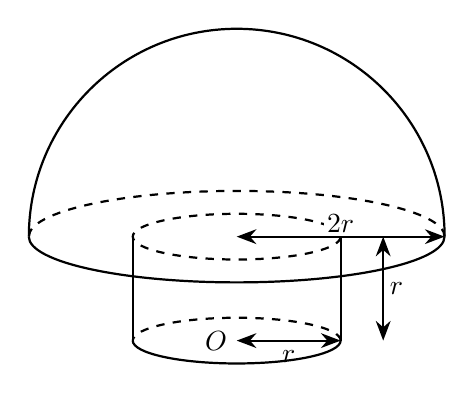
\begin{tikzpicture}[scale=1.2]
\def\rad{1.1}
\def\depthratio{0.22}
\def\dimoffset{0.45}
\pgfmathsetmacro{\height}{\rad}
\pgfmathsetmacro{\hemrad}{2*\rad}
\pgfmathsetmacro{\basedepth}{\depthratio*\rad}
\pgfmathsetmacro{\hemdepth}{\depthratio*\hemrad}
\coordinate (O) at (0,0);
\coordinate (BL) at (-\rad,0);
\coordinate (BR) at (\rad,0);
\coordinate (TL) at (-\rad,\height);
\coordinate (TR) at (\rad,\height);
\coordinate (H) at (0,\height);
\coordinate (HL) at (-\hemrad,\height);
\coordinate (HR) at (\hemrad,\height);
\coordinate (D0) at ($(BR)+(\dimoffset,0)$);
\coordinate (D1) at ($(TR)+(\dimoffset,0)$);
\draw[thick,dashed] (BR) arc[start angle=0,end angle=180,x radius=\rad,y radius=\basedepth];
\draw[thick,black] (BL) arc[start angle=180,end angle=360,x radius=\rad,y radius=\basedepth];
\draw[thick,black] (BL)--(TL);
\draw[thick,black] (BR)--(TR);
\draw[thick,dashed] (H) ellipse[x radius=\rad,y radius=\basedepth];
\draw[thick,dashed] (HR) arc[start angle=0,end angle=180,x radius=\hemrad,y radius=\hemdepth];
\draw[thick,black] (HL) arc[start angle=180,end angle=360,x radius=\hemrad,y radius=\hemdepth];
\draw[thick,black] (HR) arc[start angle=0,end angle=180,radius=\hemrad];
\draw[{Stealth[length=2.5mm]}-{Stealth[length=2.5mm]},thick] (O)--(BR) node[midway,below] {$r$};
\draw[{Stealth[length=2.5mm]}-{Stealth[length=2.5mm]},thick] (H)--(HR) node[midway,above,fill=white,inner sep=1pt] {$2r$};
\draw[{Stealth[length=2.5mm]}-{Stealth[length=2.5mm]},thick] (D0)--(D1) node[midway,right,fill=white,inner sep=2pt] {$r$};
\node[left] at (O) {$O$};
\end{tikzpicture}
\end{figure}


A composite solid $S$ consists of a uniform solid cylinder of radius $r$ and height $r$, and a uniform solid hemisphere of radius $2r$. Both components have the same density. The upper circular face of the cylinder is joined centrally to the plane face of the hemisphere, with their axes coincident and the curved surface of the hemisphere uppermost, as shown in the diagram above. The point $O$ is the centre of the lower circular face of the cylinder. \\
\begin{enumerate}[label=\textbf{(\alph*)}]
\item Find the distance from $O$ to the centre of mass of $S$, giving your answer as an exact multiple of $r$. \marks{4} \\
\end{enumerate}
The lower circular face of $S$ rests on a rough plane. The coefficient of friction between $S$ and the plane is $\mu$. Initially the plane is horizontal. Its inclination $\theta$ to the horizontal is then increased slowly, with $S$ remaining at rest until it either slides or begins to topple. No external force other than gravity and the contact force acts on $S$. \\
\begin{enumerate}[label=\textbf{(\alph*)}, resume]
\item Find the angle at which $S$ would begin to topple if sliding were prevented, giving your answer to the nearest $0.1^\circ$. Hence find the range of values of $\mu$ for which $S$ slides before it begins to topple. \marks{6} \\
\end{enumerate}

\vspace*{10pt}

\begin{djsSolution}
\begin{enumerate}[label=\textbf{(\alph*)}, start=1]
\item
By symmetry, the centre of mass \(G\) lies on the common axis. Let the common density be \(\rho\). The masses of the cylinder and hemisphere are
\begin{align*}
m_c&=\rho\pi r^2(r)=\rho\pi r^3\\
m_h&=\rho\left(\dfrac23\pi(2r)^3\right)=\dfrac{16}{3}\rho\pi r^3
\end{align*}

The centre of mass of a uniform solid cylinder lies halfway along its axis.
The centre of mass of a uniform solid hemisphere of radius \(a\) lies on its axis, a distance \(\frac38 a\) from its plane face towards the curved surface.
Thus their distances above \(O\) are
\[
x_c=\dfrac r2,\qquad x_h=r+\dfrac{3(2r)}8=\dfrac{7r}{4}
\]

For a composite solid, the centre of mass satisfies
\[
M\bar{x}=\sum m_ix_i
\]

where \(M=\sum m_i\) is the total mass. Here \(\bar{x}=OG\). Using the masses and heights above:
\begin{align*}
(m_c+m_h)OG&=m_cx_c+m_hx_h\\
\left(\rho\pi r^3+\dfrac{16}{3}\rho\pi r^3\right)OG&=\rho\pi r^3\left(\dfrac r2\right)+\dfrac{16}{3}\rho\pi r^3\left(\dfrac{7r}{4}\right)\\
\left(1+\dfrac{16}{3}\right)OG&=\left(\dfrac12+\dfrac{28}{3}\right)r\\
OG&=\dfrac{59r}{38}
\end{align*}

\item
Let \(M\) be the total mass and \(\theta_t\) the inclination at impending toppling. At the point of toppling, the vertical line through the centre of mass passes through the downhill rim of the lower circular face. The right-angled triangle formed by \(O\), the centre of mass and this rim point gives
\begin{align*}
\tan\theta_t&=\dfrac{r}{OG}=\dfrac{38}{59}\\
\theta_t&=\arctan\left(\dfrac{38}{59}\right)\approx32.8^\circ\qquad\text{(1 d.p.)}
\end{align*}

Before motion begins, let \(R\) be the normal reaction and \(F\) the frictional force acting up the plane. Resolving perpendicular and parallel to the plane gives
\[
R=Mg\cos\theta,\qquad F=Mg\sin\theta
\]

At the inclination \(\theta_s\) for impending sliding, friction is limiting, so
\begin{align*}
F&=\mu R\\
Mg\sin\theta_s&=\mu Mg\cos\theta_s\\
\tan\theta_s&=\mu
\end{align*}

\(S\) slides before it topples when \(\theta_s<\theta_t\), that is, when \(\mu<\tan\theta_t\). Hence, with \(\mu\geq0\), the required range is
\[
0\leq\mu<\dfrac{38}{59}
\]

\end{enumerate}
\end{djsSolution}

\newpage

% ---- Question 3 ----
\questionitem
% [Source: _QBT___Solns__Centre_of_Mass_of_Composite_Solids, Q3]

A solid ornament consists of a cylinder of radius $a$ and height $a$, surmounted by a cone of base radius $a$ and height $h$. Their circular faces coincide, and both parts are made from the same material of uniform density. The point $O$ is the centre of the lower circular face of the cylinder. \\

The centre of mass of the ornament is on its axis of symmetry, at a distance $\frac{9a}{10}$ above $O$. \\
\begin{enumerate}[label=\textbf{(\alph*)}]
\item Show that $h=2a$. \marks{6} \\
\end{enumerate}
A hemispherical cavity of radius $\frac{a}{2}$ is then cut into the ornament through the lower face of the cylinder. The centre of the circular opening is $O$, and the cavity extends upwards into the cylinder. \\
\begin{enumerate}[label=\textbf{(\alph*)}, resume]
\item Find the distance of the centre of mass of the remaining ornament from $O$. \marks{4} \\
\end{enumerate}
The remaining ornament is placed with its flat annular base on a rough plane. The inclination of the plane to the horizontal is slowly increased. The friction is sufficient to prevent sliding. \\
\begin{enumerate}[label=\textbf{(\alph*)}, resume]
\item Find the angle of inclination at which the ornament is on the point of toppling, giving your answer to the nearest degree. \marks{2} \\
\end{enumerate}

\vspace*{10pt}

\begin{djsSolution}
\begin{enumerate}[label=\textbf{(\alph*)}, start=1]
\item A schematic axial section is shown below, with the cavity introduced in part (b) shown dashed:\par\nopagebreak

\begin{tikzpicture}[scale=1.15, line cap=round, line join=round]
\draw (-1.5,0) -- (1.5,0) -- (1.5,1.5) -- (0,4.1) -- (-1.5,1.5) -- cycle;
\draw (-1.5,1.5) -- (1.5,1.5);
\draw[dash dot] (0,-0.2) -- (0,4.35);
\draw[dashed] (-0.75,0) arc[start angle=180,end angle=0,radius=0.75];
\node[below left] at (0,0) {$O$};
\draw[<->] (-1.95,0) -- node[left] {$a$} (-1.95,1.5);
\draw[<->] (2.0,1.5) -- node[right] {$h$} (2.0,4.1);
\draw[<->] (0,-0.5) -- node[below] {$a$} (1.5,-0.5);
\draw (0.53,0.53) -- (2.35,0.7);
\node[right,align=left] at (2.35,0.7) {Cavity of radius $\frac{a}{2}$\\in part (b)};
\end{tikzpicture}

Measure heights along the axis from \(O\), and let the uniform density be \(\rho\). For a composite solid, the centre of mass satisfies
\[
M\bar{x}=\sum m_ix_i
\]

where \(M=\sum m_i\) is the total mass.
The centre of mass of a uniform solid cylinder lies halfway along its axis.
The centre of mass of a uniform solid cone of height \(H\) lies on its axis, a distance \(\frac14 H\) from its base towards its vertex.
Thus the component heights are \(\frac{a}{2}\) and \(a+\frac{h}{4}\), respectively.

The cylinder and cone have masses \(\rho\pi a^3\) and \(\frac13\rho\pi a^2h\). Using the given centre of mass and cancelling \(\rho\pi a^2\):
\begin{align*}
\dfrac{9a}{10}\left(a+\dfrac{h}{3}\right)
&=\dfrac{a^2}{2}+\dfrac{h}{3}\left(a+\dfrac{h}{4}\right)\\
54a^2+18ah&=30a^2+20ah+5h^2\\
5h^2+2ah-24a^2&=0\\
(h-2a)(5h+12a)&=0
\end{align*}

Since \(h>0\), the negative root is inadmissible, so
\[
h=2a
\]

\item The centre of mass of a uniform solid hemisphere of radius \(R\) lies on its axis, a distance \(\frac38 R\) from its plane face towards the curved surface.
Hence the centre of mass of the removed material is at height
\[
\dfrac38\left(\dfrac a2\right)=\dfrac{3a}{16}
\]

Using \(h=2a\) from part (a), the original mass \(M\) and removed mass \(m\) are
\begin{align*}
M&=\rho\left(\pi a^3+\dfrac13\pi a^2(2a)\right)
=\dfrac53\rho\pi a^3\\
m&=\rho\left(\dfrac23\pi\left(\dfrac a2\right)^3\right)
=\dfrac1{12}\rho\pi a^3
\end{align*}

By symmetry, the remaining centre of mass is still on the axis. Using the formula from part (a), with the mass of the removed cavity counted as negative, its height \(\bar{x}\) satisfies
\begin{align*}
(M-m)\bar{x}&=M\left(\dfrac{9a}{10}\right)-m\left(\dfrac{3a}{16}\right)\\
\left(\dfrac53-\dfrac1{12}\right)\bar{x}
&=\dfrac53\left(\dfrac{9a}{10}\right)-\dfrac1{12}\left(\dfrac{3a}{16}\right)\\
\dfrac{19}{12}\bar{x}&=\dfrac{95a}{64}\\
\bar{x}&=\dfrac{15a}{16}
\end{align*}

\item Let the inclination be \(\theta\). At the point of toppling, the vertical line through the centre of mass passes through the downhill outer rim of the annular base. The right-angled triangle formed by \(O\), the centre of mass and this rim point gives
\[
\tan\theta=\dfrac{a}{\bar{x}}=\dfrac{16}{15}
\]

Therefore the required inclination is
\[
\theta=\arctan\left(\dfrac{16}{15}\right)\approx47^\circ
\qquad\text{(nearest degree)}
\]

\end{enumerate}
\end{djsSolution}

\newpage

% ---- Question 4 ----
\questionitem
% [Source: _QBT___Solns__Centre_of_Mass_of_Composite_Solids, Q4]

\begin{figure}[H]
    \centering
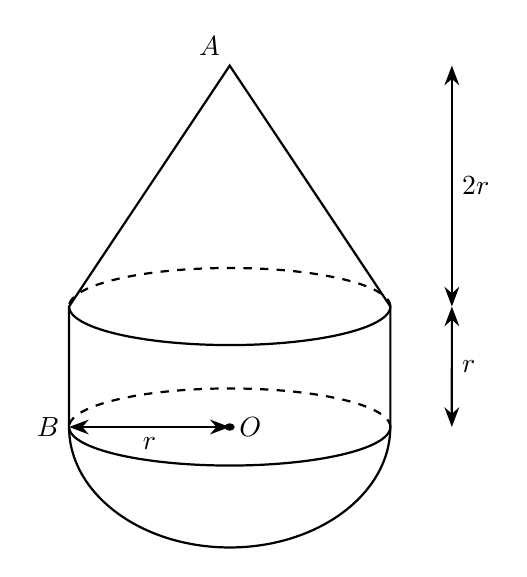
\begin{tikzpicture}[scale=1.2, yscale=0.75]
\def\rad{1.7}
\def\ellipseRatio{0.32}
\def\cylFactor{1}
\def\coneFactor{2}
\def\dimOffset{0.65}
\pgfmathsetmacro{\cylHeight}{\cylFactor*\rad}
\pgfmathsetmacro{\totalHeight}{(\cylFactor+\coneFactor)*\rad}
\coordinate (O) at (0,0);
\coordinate (B) at (-\rad,0);
\coordinate (R) at (\rad,0);
\coordinate (Ltop) at (-\rad,\cylHeight);
\coordinate (Rtop) at (\rad,\cylHeight);
\coordinate (A) at (0,\totalHeight);
\coordinate (Dbase) at ($(R)+(\dimOffset,0)$);
\coordinate (Djoin) at (Dbase |- Rtop);
\coordinate (Dtop) at (Dbase |- A);
\draw[thick, black] (B) -- (Ltop) -- (A) -- (Rtop) -- (R);
\foreach \height in {0,\cylHeight} {
  \draw[dashed, thick, black] plot[domain=0:180, samples=80] ({\rad*cos(\x)},{\height+\ellipseRatio*\rad*sin(\x)});
  \draw[thick, black] plot[domain=180:360, samples=80] ({\rad*cos(\x)},{\height+\ellipseRatio*\rad*sin(\x)});
}
\draw[thick, black] (B) arc[start angle=180, end angle=360, radius=\rad];
\draw[{Stealth[length=2.5mm]}-{Stealth[length=2.5mm]}, thick, black] (B) -- (O) node[midway, below] {$r$};
\draw[{Stealth[length=2.5mm]}-{Stealth[length=2.5mm]}, thick, black] (Dbase) -- (Djoin) node[midway, right] {$r$};
\draw[{Stealth[length=2.5mm]}-{Stealth[length=2.5mm]}, thick, black] (Djoin) -- (Dtop) node[midway, right] {$2r$};
\fill[black] (O) circle (1.5pt);
\node[above left] at (A) {$A$};
\node[left] at (B) {$B$};
\node[right] at (O) {$O$};
\end{tikzpicture}
\end{figure}


A composite solid is made from a solid hemisphere, a solid cylinder and a solid right circular cone, all made from the same material of uniform density. Each component has radius $r$. The cylinder has height $r$ and the cone has height $2r$. \\

The plane face of the hemisphere is joined to one circular face of the cylinder, and the base of the cone is joined to the other circular face of the cylinder. Their axes coincide, as shown in the diagram above. The centre of the common face of the hemisphere and cylinder is $O$, and $B$ lies on its circumference, with $OB=r$. \\
\begin{enumerate}[label=\textbf{(\alph*)}]
\item Find the distance of the centre of mass of the composite solid from $O$, stating on which side of $O$ it lies. \marks{4} \\
\end{enumerate}
The cone is now removed and replaced by a solid right circular cone of base radius $r$ and height $hr$, where $h>0$, made from the same material. The hemisphere and cylinder are unchanged. This new composite solid is suspended by a light string attached to $B$ and hangs freely in equilibrium. The acute angle between $OB$ and the vertical is $45^\circ$. \\
\begin{enumerate}[label=\textbf{(\alph*)}, resume]
\item Find the exact value of $h$. \marks{4} \\
\end{enumerate}

\vspace*{10pt}

\begin{djsSolution}
\begin{enumerate}[label=\textbf{(\alph*)}, start=1]
\item
Take the common axis as the \(x\)-axis, with origin \(O\) and positive direction towards \(A\). By symmetry, the centre of mass lies on this axis. Let the common density be \(\rho\).

The centre of mass of a uniform solid hemisphere of radius \(R\) lies on its axis, a distance \(\frac38 R\) from its plane face towards the curved surface.
The centre of mass of a uniform solid cylinder lies halfway along its axis.
The centre of mass of a uniform solid cone of height \(H\) lies on its axis, a distance \(\frac14 H\) from its base towards its vertex.
Using mass \(=\) density \(\times\) volume:
\[
\begingroup
\renewcommand{\arraystretch}{1.65}
\setlength{\arraycolsep}{10pt}
\begin{array}{c|c|c}
\text{Component} & \text{Mass} & \text{Axial coordinate} \\
\hline
\text{Hemisphere} & \frac{2}{3}\rho\pi r^3 & -\frac{3r}{8} \\
\text{Cylinder} & \rho\pi r^3 & \frac{r}{2} \\
\text{Cone} & \frac{2}{3}\rho\pi r^3 & r+\frac{2r}{4}=\frac{3r}{2}
\end{array}
\endgroup
\]

For a composite solid, the centre of mass satisfies
\[
M\bar{x}=\sum m_ix_i
\]

where \(M=\sum m_i\) is the total mass. Substituting the masses and positions:
\begin{align*}
\left(\dfrac{2}{3}+1+\dfrac{2}{3}\right)\rho\pi r^3\bar{x}
&=\dfrac{2}{3}\rho\pi r^3\left(-\dfrac{3r}{8}\right)
+\rho\pi r^3\left(\dfrac{r}{2}\right)
+\dfrac{2}{3}\rho\pi r^3\left(\dfrac{3r}{2}\right) \\
\dfrac{7}{3}\rho\pi r^3\bar{x}
&=\left(-\dfrac{1}{4}+\dfrac{1}{2}+1\right)\rho\pi r^4 \\
\bar{x}&=\dfrac{15r}{28}
\end{align*}

This coordinate is positive, so the required distance and side are
\[
\dfrac{15r}{28},\qquad \text{on the cylinder and cone side of }O
\]

\item
Let the new centre of mass be \(G'\), with signed axial coordinate \(\bar{x}'\). The replacement cone has mass \(\frac{h}{3}\rho\pi r^3\) and its centre of mass is at \(r+\frac{hr}{4}\).

Using the centre-of-mass formula from part (a):
\begin{align*}
\dfrac{5+h}{3}\rho\pi r^3\bar{x}'
&=-\dfrac{1}{4}\rho\pi r^4+\dfrac{1}{2}\rho\pi r^4
+\dfrac{h}{3}\rho\pi r^3\left(r+\dfrac{hr}{4}\right) \\
&=\dfrac{\rho\pi r^4}{12}\left(3+4h+h^2\right)
\end{align*}

Since \(h>0\), the right-hand side is positive, so \(G'\) lies on the positive side of \(O\).

When the solid hangs freely in equilibrium, \(G'\) is vertically below \(B\). Also, \(OB\) is perpendicular to \(OG'\), so the right-angled triangle \(BOG'\) gives
\[
\tan45^\circ=\dfrac{OG'}{OB}=\dfrac{\bar{x}'}{r}
\quad\Longrightarrow\quad \bar{x}'=r
\]

Substituting into the moment equation and cancelling \(\rho\pi r^4\):
\begin{align*}
\dfrac{5+h}{3}&=\dfrac{3+4h+h^2}{12} \\
4(5+h)&=3+4h+h^2 \\
h^2&=17 \\
h&=\sqrt{17}\qquad(h>0)
\end{align*}

\end{enumerate}
\end{djsSolution}

\newpage

% ---- Question 5 ----
\questionitem
% [Source: _QBT___Solns__Centre_of_Mass_of_Composite_Solids, Q5]

\begin{figure}[H]
\centering
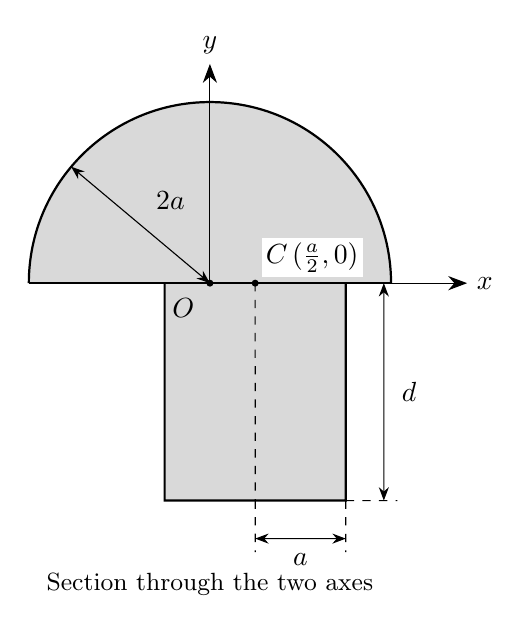
\begin{tikzpicture}[scale=1.15,
  outline/.style={thick,black},
  dimension/.style={{Stealth[length=1.7mm]}-{Stealth[length=1.7mm]},black},
  every node/.style={font=\normalsize}]
\def\a{1}
\def\heightRatio{2.4}
\def\radiusAngle{140}
\pgfmathsetmacro{\hemrad}{2*\a}
\pgfmathsetmacro{\height}{\heightRatio*\a}
\pgfmathsetmacro{\offset}{\a/2}
\pgfmathsetmacro{\gap}{0.42*\a}
\coordinate (O) at (0,0);
\coordinate (C) at (\offset,0);
\coordinate (HL) at (-\hemrad,0);
\coordinate (HR) at (\hemrad,0);
\coordinate (HT) at (0,\hemrad);
\coordinate (CL) at ($(C)+(-\a,0)$);
\coordinate (CR) at ($(C)+(\a,0)$);
\coordinate (B) at ($(C)+(0,-\height)$);
\coordinate (BL) at ($(B)+(-\a,0)$);
\coordinate (BR) at ($(B)+(\a,0)$);
\coordinate (P) at (\radiusAngle:\hemrad);
\coordinate (X) at ($(HR)+(2*\gap,0)$);
\coordinate (Y) at ($(HT)+(0,\gap)$);
\coordinate (Dtop) at ($(CR)+(\gap,0)$);
\coordinate (Dbottom) at ($(BR)+(\gap,0)$);
\coordinate (Rstart) at ($(B)+(0,-\gap)$);
\coordinate (Rend) at ($(BR)+(0,-\gap)$);
\coordinate (Title) at ($(O)+(0,-\height-2.2*\gap)$);
\fill[gray!30] (HR) arc[start angle=0,end angle=180,radius=\hemrad] -- cycle;
\fill[gray!30] (CL) -- (BL) -- (BR) -- (CR) -- cycle;
\draw[outline] (HR) arc[start angle=0,end angle=180,radius=\hemrad];
\draw[outline] (HL) -- (HR);
\draw[outline] (CL) -- (BL) -- (BR) -- (CR);
\draw[black,-{Stealth[length=2.4mm]}] (O) -- (X) node[right] {$x$};
\draw[black,-{Stealth[length=2.4mm]}] (O) -- (Y) node[above] {$y$};
\draw[black,dashed] (C) -- (B);
\draw[dimension] (O) -- node[midway,above right=3pt] {$2a$} (P);
\draw[black,dashed] (CR) -- ($(Dtop)+(0.15*\a,0)$);
\draw[black,dashed] (BR) -- ($(Dbottom)+(0.15*\a,0)$);
\draw[dimension] (Dtop) -- node[midway,right=3pt] {$d$} (Dbottom);
\draw[black,dashed] (B) -- ($(Rstart)+(0,-0.15*\a)$);
\draw[black,dashed] (BR) -- ($(Rend)+(0,-0.15*\a)$);
\draw[dimension] (Rstart) -- node[midway,below=2pt] {$a$} (Rend);
\fill[black] (O) circle (1.1pt);
\fill[black] (C) circle (1.1pt);
\node[below left=3pt] at (O) {$O$};
\node[above right=3pt,fill=white,inner sep=1.5pt] at (C) {$C\,(\tfrac a2,0)$};
\node[font=\small] at (Title) {Section through the two axes};
\end{tikzpicture}
\end{figure}


A composite solid consists of a solid hemisphere of radius $2a$ and a solid cylinder of radius $a$ and height $d$, where $a>0$ and $d>0$. Both components have the same uniform density. \\

The cylinder is attached below the plane face of the hemisphere, as shown in the diagram above. The centre of this plane face is $O$. The axis of the cylinder meets the plane face at $C$, where $OC=\frac{a}{2}$. The $x$-axis is directed from $O$ towards $C$, and the $y$-axis is directed into the hemisphere, perpendicular to its plane face. \\
\begin{enumerate}[label=\textbf{(\alph*)}]
\item Find the coordinates $(\bar{x},\bar{y})$ of the centre of mass of the composite solid in terms of $a$ and $d$. \marks{5} \\
\end{enumerate}
The solid is now placed with the lower circular face of the cylinder on a rough plane inclined at an angle $\theta$ to the horizontal, where $\tan\theta=\frac{1}{2}$. The positive $x$-direction points directly down the line of greatest slope, and the positive $y$-direction is perpendicular to the plane and away from it. The plane is sufficiently rough to prevent sliding. \\
\begin{enumerate}[label=\textbf{(\alph*)}, resume]
\item Find the greatest value of $d$ for which the solid can rest without toppling. Give your answer as an exact multiple of $a$. \marks{4} \\
\end{enumerate}

\vspace*{10pt}

\begin{djsSolution}
\begin{enumerate}[label=\textbf{(\alph*)}, start=1]
\item
Let the common density be \(\rho\), and let the masses of the hemisphere and cylinder be \(m_h\) and \(m_c\). Using their standard volume formulae:
\[
m_h=\rho\left(\frac23\pi(2a)^3\right)=\frac{16}{3}\rho\pi a^3,
\qquad
m_c=\rho\pi a^2d
\]

The centre of mass of a uniform solid hemisphere of radius \(R\) lies on its axis, a distance \(\frac38 R\) from its plane face towards the curved surface.
The centre of mass of a uniform solid cylinder lies halfway along its axis.
Thus the component centres are
\[
H\left(0,\frac{3a}{4}\right),
\qquad
K\left(\frac a2,-\frac d2\right)
\]

For a composite solid, the centre of mass satisfies
\[
M\bar{x}=\sum m_ix_i,
\qquad
M\bar{y}=\sum m_iy_i
\]

where \(M=\sum m_i\) is the total mass. Substituting and cancelling the common factor \(\rho\pi a^2\):
\begin{align*}
\left(\dfrac{16a}{3}+d\right)\bar{x}&=\dfrac{16a}{3}(0)+d\left(\dfrac a2\right)\\
\bar{x}&=\dfrac{3ad}{2(16a+3d)}\\
\left(\dfrac{16a}{3}+d\right)\bar{y}&=\dfrac{16a}{3}\left(\dfrac{3a}{4}\right)+d\left(-\dfrac d2\right)\\
\bar{y}&=\dfrac{24a^2-3d^2}{2(16a+3d)}
\end{align*}

Hence the required coordinates are
\[
(\bar{x},\bar{y})
=\left(\frac{3ad}{2(16a+3d)},\frac{24a^2-3d^2}{2(16a+3d)}\right)
\]

\item The downhill rim of the cylinder has \(x\)-coordinate \(\frac a2+a=\frac{3a}{2}\). Both component centres lie downhill of the uphill rim, so only downhill toppling is possible.

The centre of mass is \(d+\bar{y}\) above the plane, and \(\frac{3a}{2}-\bar{x}\) up the slope from the downhill rim. At the point of toppling, the vertical line through the centre of mass passes through the downhill rim, so the solid rests without toppling when
\[
\tan\theta\leq\dfrac{\dfrac{3a}{2}-\bar{x}}{d+\bar{y}}
\]

Using part (a):
\begin{align*}
\dfrac{3a}{2}-\bar{x}&=\dfrac{3a}{2}-\dfrac{3ad}{2(16a+3d)}=\dfrac{48a^2+6ad}{2(16a+3d)}\\
d+\bar{y}&=d+\dfrac{24a^2-3d^2}{2(16a+3d)}=\dfrac{3d^2+32ad+24a^2}{2(16a+3d)}
\end{align*}

Substituting these and \(\tan\theta=\frac12\), then multiplying by the positive denominators:
\begin{align*}
\dfrac12&\leq\dfrac{48a^2+6ad}{3d^2+32ad+24a^2}\\
3d^2+32ad+24a^2&\leq 96a^2+12ad\\
3d^2+20ad-72a^2&\leq 0
\end{align*}

Since \(a>0\) and \(d>0\), the greatest permitted height is the positive root, where toppling is just about to occur:
\[
d_{\max}=\frac{-20a+\sqrt{(20a)^2+4(3)(72a^2)}}{6}
=\frac{2\sqrt{79}-10}{3}\,a
\]

\end{enumerate}
\end{djsSolution}

\newpage

% ---- Question 6 ----
\questionitem
% [Source: _QBT___Solns__Centre_of_Mass_of_Composite_Solids, Q6]

\begin{figure}[H]
    \centering
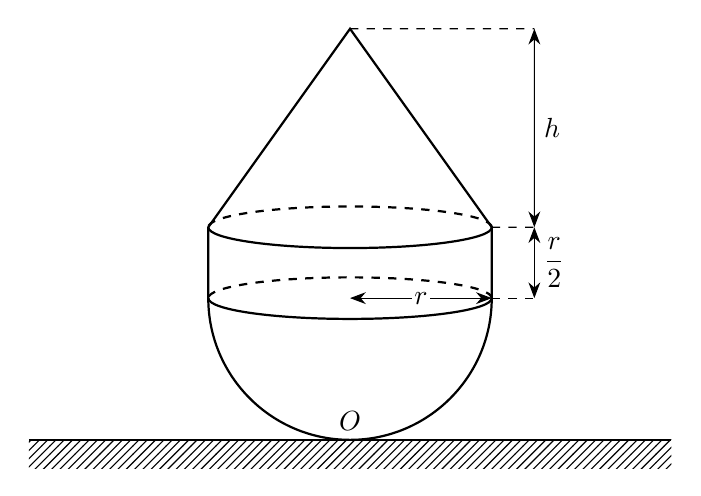
\begin{tikzpicture}[scale=1.2]
\def\rad{1.5}
\def\coneHeight{2.1}
\def\ellipseDepth{0.22}
\def\groundExtent{3.4}
\def\groundDepth{0.3}
\def\dimOffset{0.45}
\pgfmathsetmacro{\cylHeight}{\rad/2}
\coordinate (C) at (0,0);
\coordinate (T) at (0,\cylHeight);
\coordinate (V) at ($(T)+(0,\coneHeight)$);
\coordinate (O) at (0,-\rad);
\coordinate (L) at (-\rad,0);
\coordinate (R) at (\rad,0);
\coordinate (TL) at ($(T)+(-\rad,0)$);
\coordinate (TR) at ($(T)+(\rad,0)$);
\coordinate (D0) at ($(R)+(\dimOffset,0)$);
\coordinate (D1) at ($(TR)+(\dimOffset,0)$);
\coordinate (D2) at (D1 |- V);
\fill[pattern=north east lines] (-\groundExtent,{-\rad-\groundDepth}) rectangle (\groundExtent,-\rad);
\draw[thick,black] (-\groundExtent,-\rad) -- (\groundExtent,-\rad);
\draw[thick,black] (L) arc[start angle=180,end angle=360,radius=\rad];
\draw[thick,black] (L) -- (TL) -- (V) -- (TR) -- (R);
\foreach \P in {C,T} {
  \draw[thick,black,dashed] ($(\P)+(\rad,0)$) arc[start angle=0,end angle=180,x radius=\rad,y radius=\ellipseDepth];
  \draw[thick,black] ($(\P)+(-\rad,0)$) arc[start angle=180,end angle=360,x radius=\rad,y radius=\ellipseDepth];
}
\draw[{Stealth[length=2mm]}-{Stealth[length=2mm]}] (C) -- node[midway,fill=white,inner sep=1pt] {$r$} (R);
\draw[dashed] (R) -- (D0);
\draw[dashed] (TR) -- (D1);
\draw[dashed] (V) -- (D2);
\draw[{Stealth[length=2mm]}-{Stealth[length=2mm]}] (D0) -- node[midway,right] {$\dfrac r2$} (D1);
\draw[{Stealth[length=2mm]}-{Stealth[length=2mm]}] (D1) -- node[midway,right] {$h$} (D2);
\node[above] at (O) {$O$};
\end{tikzpicture}
\end{figure}


A self-righting ornament is formed by joining a solid hemisphere, a solid cylinder and a solid cone, as shown in the diagram above. All three components are made from the same material of uniform density and have a common axis of symmetry. \\

The hemisphere has radius $r$. The cylinder has radius $r$ and height $\frac{r}{2}$, and its lower face coincides with the plane face of the hemisphere. The cone has base radius $r$ and height $h$, and its base coincides with the upper face of the cylinder. \\

The ornament rests on a horizontal plane at the lowest point $O$ of the hemisphere, with its axis vertical and the cone uppermost. \\

You may use the following results for uniform solids:
\begin{itemize}[nosep]
\item A hemisphere of radius $r$ has volume $\frac{2}{3}\pi r^3$ and its centre of mass is $\frac38 r$ from its plane face towards its curved surface.
\item A cone of base radius $r$ and height $h$ has volume $\frac{1}{3}\pi r^2h$ and its centre of mass is $\frac14 h$ from its base towards its vertex.
\end{itemize}
\begin{enumerate}[label=\textbf{(\alph*)}]
\item Find, in terms of $r$ and $h$, the distance $d$ of the centre of mass of the ornament from $O$. Simplify your answer. \marks{5} \\
\item Find the exact range of values of $\frac{h}{r}$ for which the ornament is in stable equilibrium in this position, so that it tends to return towards the vertical after a small tilt. \marks{4} \\
\end{enumerate}

\vspace*{10pt}

\begin{djsSolution}
\begin{enumerate}[label=\textbf{(\alph*)}, start=1]
\item
By symmetry, the centre of mass lies on the common axis. Let \(\rho\) be the common density, and measure heights vertically upwards from \(O\).

The centre of mass of a uniform solid hemisphere of radius \(R\) lies on its axis, a distance \(\frac38 R\) from its plane face towards the curved surface.
The centre of mass of a uniform solid cylinder lies halfway along its axis.
The centre of mass of a uniform solid cone of height \(H\) lies on its axis, a distance \(\frac14 H\) from its base towards its vertex.
Using mass \(=\) density \(\times\) volume:
\[
\begingroup
\renewcommand{\arraystretch}{1.65}
\setlength{\arraycolsep}{10pt}
\begin{array}{c|c|c}
\text{Component} & \text{Mass }m_i & \text{Height }x_i\text{ above }O\\ \hline
\text{Hemisphere} & \rho\left(\frac23\pi r^3\right)
& r-\frac{3r}{8}=\frac{5r}{8}\\
\text{Cylinder} & \rho\left(\pi r^2\times\frac r2\right)
& r+\frac r4=\frac{5r}{4}\\
\text{Cone} & \rho\left(\frac13\pi r^2h\right)
& r+\frac r2+\frac h4=\frac{3r}{2}+\frac h4
\end{array}
\endgroup
\]

For a composite solid, the centre of mass satisfies
\[
M\bar{x}=\sum m_ix_i
\]

where \(M=\sum m_i\) is the total mass. Here \(\bar{x}=d\).

Substituting and cancelling the common factor \(\rho\pi r^2\):
\begin{align*}
\left(\dfrac{2r}{3}+\dfrac r2+\dfrac h3\right)d
&=\dfrac{2r}{3}\times\dfrac{5r}{8}
+\dfrac r2\times\dfrac{5r}{4}
+\dfrac h3\left(\dfrac{3r}{2}+\dfrac h4\right)\\
\dfrac{7r+2h}{6}\,d
&=\dfrac{5r^2}{12}+\dfrac{5r^2}{8}+\dfrac{rh}{2}+\dfrac{h^2}{12}\\
&=\dfrac{25r^2+12rh+2h^2}{24}\\
d&=\dfrac{25r^2+12rh+2h^2}{4(7r+2h)}
\end{align*}

\item Let \(C\) be the centre of the hemisphere, so \(OC=r\). After a small tilt, the weight produces a restoring moment about the point of contact precisely when the centre of mass is below \(C\). If it coincides with \(C\), there is no restoring moment, so stable equilibrium requires the strict inequality \(d<r\).

Using part (a), with \(r>0\) and \(h>0\):
\begin{align*}
\dfrac{25r^2+12rh+2h^2}{4(7r+2h)}&<r\\
25r^2+12rh+2h^2&<28r^2+8rh\\
2h^2+4rh-3r^2&<0\\
2\left(\dfrac hr\right)^2+4\left(\dfrac hr\right)-3&<0\\
\left(\dfrac hr+1\right)^2&<\dfrac52
\end{align*}

Since \(\frac hr>0\), the required exact range is
\[
0<\dfrac hr<\sqrt{\dfrac52}-1=\dfrac{\sqrt{10}-2}{2}
\]

\end{enumerate}
\end{djsSolution}

\end{enumerate}
\end{document}
